\section{Background}

%%%%%%%%%%%%%%%%%%%%%%%%%%%%%%%%%%%%%%%%%%%%%%%%%%%%%%%%%%%%%%%%%%%%%%%%%%%%%%
\subsection{Message Passing}

\begin{slide}
    \begin{center}A Taxonomy of Message-Passing:\end{center}
    \begin{figure}[htp]
    \centering
    \Tree [ .{Message Passing}
			[ .Async 
				Direct 
				Indirect 
			] 
			[ .Sync 
				Asymmetric
				Symmetric 
			]
	   ]
    \label{fig:mptax}
    \end{figure}

    \note{
        \begin{itemize}
            \item Async: while user code doesn't block, there is blocking
                    in terms of the channel implementation. This is not
                    indicated (in most cases) to the scheduler.
            \item Direct = Mailboxes
            \item Indirect = Sockets
            \item Sync: The issue of process cooperation has been elevated
                    to the process level for the scheduler to directly involve
                    itself.
        \end{itemize}
    }
\end{slide}

\begin{slide}
    \begin{center} {\Large swap} \end{center}
    Our Symmetric Synchronous Message Passing Primitive
    \begin{itemize}
        \item Purely captures cooperation of processes by synchronizing on
                the shared channel.
        \item Ultimately can be extended to take into account:
            \begin{itemize}
                \item Directionality
                \item Asynchrony
            \end{itemize}
    \end{itemize}
    \note{
        Ultimately there is nothing stopping us from choosing the other
        types of message passing, but it would conflate the issue of
        process cooperativity if all we are after is whether two processes
        are cooperating on some task.
    }
\end{slide}

%%%%%%%%%%%%%%%%%%%%%%%%%%%%%%%%%%%%%%%%%%%%%%%%%%%%%%%%%%%%%%%%%%%%%%%%%%%%%%
\subsection{Cooperativity}

\begin{slide}
    \begin{figure} 
    \centering
        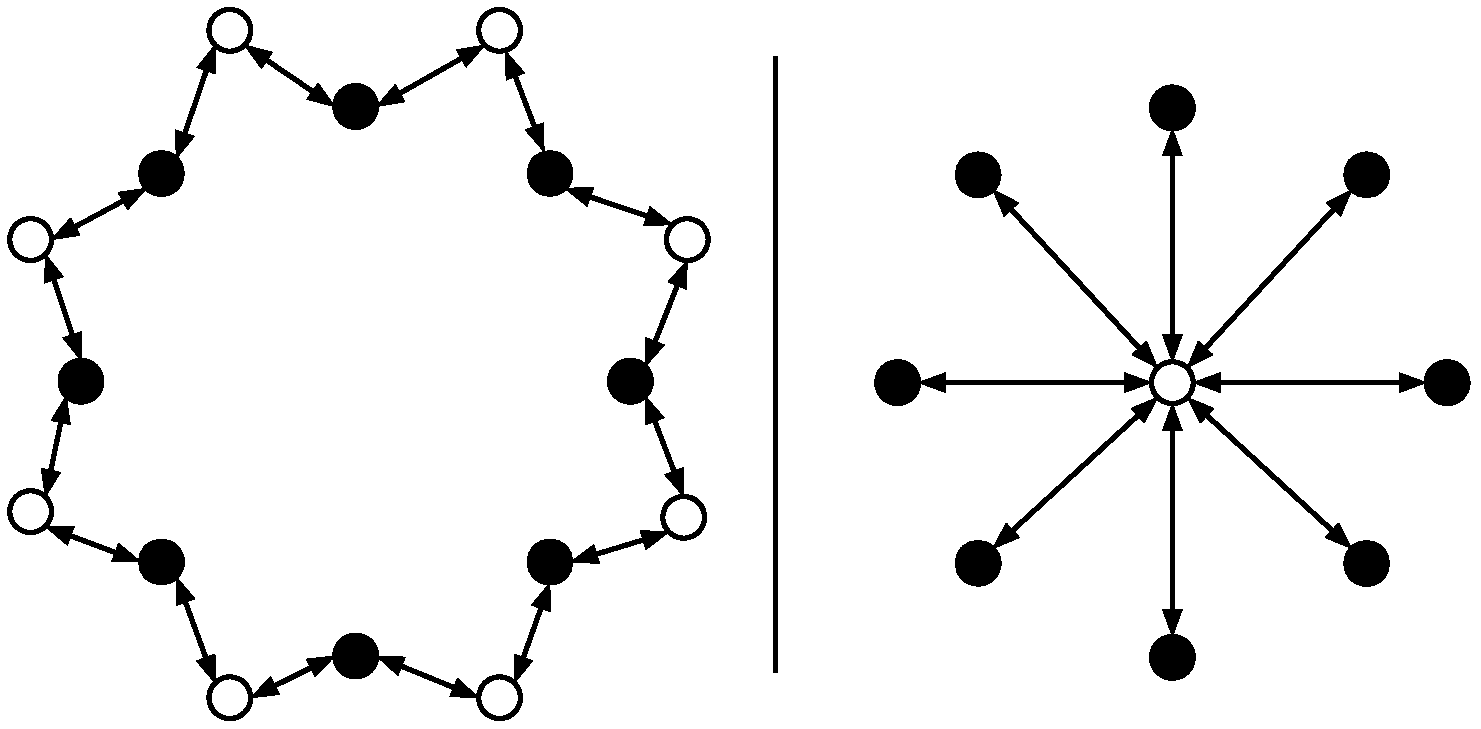
\includegraphics[scale=0.4]{RingVCluster.pdf}
        \label{fig:RingVCluster}
    \end{figure}

    \note{
        Whats the difference in cooperativity in the left and right
        set of processes? Where white represents a channel and black 
        represents a process.
        \begin{itemize}
            \item Left: A Ring, the level of parallelism is nearly nil. Each
                process is cooperating yes, but the granularity of the 
                application is very fine.

            \item Right: A Star, the level of parallelism is nearly full. Each
                process is cooperating, and is not reliant on more than one 
                other.
        \end{itemize}
        Overall, what can be gained by looking at cooperativity in terms of
        understanding the applications behaviour? Knowing the granularity of
        parallelism.
    }
\end{slide}


%%%%%%%%%%%%%%%%%%%%%%%%%%%%%%%%%%%%%%%%%%%%%%%%%%%%%%%%%%%%%%%%%%%%%%%%%%%%%%
\subsection{Runtime Scheduling}

%\begin{slide}
%    \begin{itemize}
%        \item Simple Step Scheduling
%        \item Continuous to Discrete Translation
%    \end{itemize}
%    \inote{
%        \item Runtime scheduling is a big topic.
%        \item Focus on how we translated scheduling into our API 
%    }
%\end{slide}
%
%\begin{slide}
%    Term List:
%    \begin{itemize}
%        \item Round-Robin
%        \item Time-Quantum
%        \item Work-Stealing
%    \end{itemize}
%    
%\end{slide}

\begin{slide}
%    Feedback Scheduling:

    \inote{
        \item How much of basic runtime scheduling do I need to talk about 
            here? I may want to save it until Schedulers section and just
            discuss it all there.
    }
\end{slide}

